\documentclass[compress]{beamer}
\usepackage{ifthen,verbatim}

\newcommand{\isnote}{}
\xdefinecolor{lightyellow}{rgb}{1.,1.,0.25}
\xdefinecolor{darkblue}{rgb}{0.1,0.1,0.7}

%% Uncomment this to get annotations
%% \def\notes{\addtocounter{page}{-1}
%%            \renewcommand{\isnote}{*}
%% 	   \beamertemplateshadingbackground{lightyellow}{white}
%%            \begin{frame}
%%            \frametitle{Notes for the previous page (page \insertpagenumber)}
%%            \itemize}
%% \def\endnotes{\enditemize
%% 	      \end{frame}
%%               \beamertemplateshadingbackground{white}{white}
%%               \renewcommand{\isnote}{}}

%% Uncomment this to not get annotations
\def\notes{\comment}
\def\endnotes{\endcomment}

\setbeamertemplate{navigation symbols}{}
\setbeamertemplate{headline}{\mbox{ } \hfill
\begin{minipage}{5.5 cm}
\vspace{-0.75 cm} \small
\end{minipage} \hfill
\begin{minipage}{4.5 cm}
\vspace{-0.75 cm} \small
\begin{flushright}
\ifthenelse{\equal{\insertpagenumber}{1}}{}{Jim Pivarski \hspace{0.2 cm} \insertpagenumber\isnote/\pageref{numpages}}
\end{flushright}
\end{minipage}\mbox{\hspace{0.2 cm}}\includegraphics[height=1 cm]{../cmslogo} \hspace{0.01 cm} \vspace{-1.05 cm}}

\begin{document}
\begin{frame}
\vfill
\begin{center}
\textcolor{darkblue}{\Large Muon Alignment News}

\vfill
\begin{columns}
\column{0.75\linewidth}
\begin{center}
\large
Jim Pivarski \hspace{0.5 cm} Gervasio Gomez
\end{center}
\end{columns}

\vfill
 3 September, 2010

\end{center}
\end{frame}

%% \begin{notes}
%% \item This is the annotated version of my talk.
%% \item If you want the version that I am presenting, download the one
%% labeled ``slides'' on Indico (or just ignore these yellow pages).
%% \item The annotated version is provided for extra detail and a written
%% record of comments that I intend to make orally.
%% \item Yellow notes refer to the content on the {\it previous} page.
%% \item All other slides are identical for the two versions.
%% \end{notes}

\small

\begin{frame}
\frametitle{Outline}
\begin{itemize}\setlength{\itemsep}{0.75 cm}
\item Alignment documentation
\item Proposal to collect beam-halo only for special runs
\item Upcoming alignment update: endcap disks w.r.t.\ tracker
\end{itemize}
%% \hspace{-0.83 cm} \textcolor{darkblue}{\Large Outline2}
\end{frame}

\begin{frame}
\frametitle{Alignment documentation}
\framesubtitle{Many different twiki pages!}

\begin{itemize}
\item MuonAlignment: \href{https://twiki.cern.ch/twiki/bin/view/CMS/MuonAlignment}{\tt \tiny \textcolor{blue}{https://twiki.cern.ch/twiki/bin/view/CMS/MuonAlignment}}
\begin{itemize}
\item general introduction with a few plots from MTCC \textcolor{darkblue}{(2006)}
\item fully described pre-CRUZET Millepede results \textcolor{darkblue}{(2007)}, CRUZET endcap disk alignments with HIP-Ntuple \textcolor{darkblue}{(2008)}, \\ new hardware endcap alignment \textcolor{darkblue}{(2010)}
\end{itemize}

\item SWGuideAlignmentConstants: \href{https://twiki.cern.ch/twiki/bin/view/CMS/SWGuideAlignmentConstants}{\tt \tiny \textcolor{blue}{.../SWGuideAlignmentConstants}}
\begin{itemize}
\item fully described tracker and muon alignments from TIF/MTCC era through end of CRAFT era \textcolor{darkblue}{(2006--Mar 2010)}
\item overlaps with MuonAlignment but more complete
\item fully described tracker and muon MC misalignment scenarios
\end{itemize}

\item AlCaScenarios: \href{https://twiki.cern.ch/twiki/bin/view/CMS/AlCaScenarios}{\tt \tiny \textcolor{blue}{.../AlCaScenarios}}
\begin{itemize}
\item tracker and muon misalignment scenarios (overlaps SWGuideAlignmentConstants)
\end{itemize}

\item SWGuideMuonAlignment: \href{https://twiki.cern.ch/twiki/bin/view/CMS/SWGuideMuonAlignment}{\tt \tiny \textcolor{blue}{.../SWGuideMuonAlignment}}
\begin{itemize}
\item software tools for doing track-based alignments and making validation plots; not a place for alignment results
\end{itemize}

\end{itemize}
\end{frame}

\begin{frame}
\frametitle{Alignment Documentation}
\begin{itemize}
\item Looked up tags using Pablo's hn-cms-alca e-mail and \href{https://twiki.cern.ch/twiki/bin/view/CMS/SWGuideFrontierConditions}{\tt \textcolor{blue}{SWGuideFrontierConditions}} twiki page

\item All in {\tt \tiny frontier://PromptProd/CMS\_COND\_31X\_ALIGNMENT} and GR10\_E\_V9 GlobalTag

\begin{tabular}{l l l}
\tiny Type & \tiny Latest tag name & \tiny Latest IOV \\\hline
\tiny GlobalPositionRcd & \tiny GlobalAlignment\_2009\_v2\_express & \tiny 1--$\infty$ \\
\tiny DTAlignmentRcd & \tiny DTAlignment\_2009\_v1\_express & \tiny 137353--$\infty$ \\
\tiny CSCAlignmentRcd & \tiny CSCAlignment\_2009\_v2\_express & \tiny 1--$\infty$ \\
\tiny DTAlignmentErrorRcd & \tiny DTAlignmentError\_2009\_v1\_express & \tiny 137353--$\infty$ \\
\tiny CSCAlignmentErrorRcd & \tiny CSCAlignmentError\_2009\_v1\_express & \tiny 133193--$\infty$ \\
\end{tabular}

\item Comprehensive HW barrel alignment documentation?

\item New alignment, consequences of TB-HW uncertainty on $Z'$ \href{http://indico.cern.ch/contributionDisplay.py?contribId=5&sessionId=1&confId=103403}{\tt \tiny \textcolor{blue}{http://indico.cern.ch/contributionDisplay.py?contribId=5\&sessionId=1\&confId=103403}}

\item Beam-halo/endcaps: \href{http://indico.cern.ch/contributionDisplay.py?contribId=6&confId=94861}{\tt \tiny \textcolor{blue}{http://indico.cern.ch/contributionDisplay.py?contribId=6\&confId=94861}}
\href{http://indico.cern.ch/contributionDisplay.py?contribId=4&confId=94196}{\tt \tiny \textcolor{blue}{http://indico.cern.ch/contributionDisplay.py?contribId=4\&confId=94196}}
\href{https://hypernews.cern.ch/HyperNews/CMS/get/muon-alignment/533/1.html}{\tt \tiny \textcolor{blue}{https://hypernews.cern.ch/HyperNews/CMS/get/muon-alignment/533/1.html}}

\item Luca's validation: \href{http://indico.cern.ch/subContributionDisplay.py?subContId=0&contribId=3&confId=104241}{\tt \tiny \textcolor{blue}{http://indico.cern.ch/subContributionDisplay.py?subContId=0\&contribId=3\&confId=104241}}

\end{itemize}
\end{frame}

\begin{frame}
\frametitle{Alignment data streams}
\begin{itemize}
\item \textcolor{darkblue}{MuAlCalIsolatedMu:} GlobalMuons, TrackerMuons, and StandAloneMuons in collisions

\item \textcolor{darkblue}{MuAlGlobalCosmics:} barrel GlobalMuons for cosmics runs

\item \textcolor{darkblue}{MuAlBeamHaloOverlaps and HLT\_CSCBeamHaloOverlaps*:} still collecting beam-halo data for alignment
\begin{itemize}
\item starting to limit bandwidth for physics
\item we seem to only need to align once after a shut-down
\item most useful when we request a beam-halo burst from the LHC, anyway
\end{itemize}
\end{itemize}

\vfill
\hspace{-0.83 cm} \textcolor{darkblue}{\Large Proposal}

\vspace{0.1 cm}
\begin{itemize}
\item Drop beam-halo AlCaReco and associated trigger from normal data-taking stream
\item Only request special beam-halo runs after a shut-down and every few months
\end{itemize}
\end{frame}

%% \section*{First section}
%% \begin{frame}
%% \begin{center}
%% \Huge \textcolor{blue}{First section}
%% \end{center}
%% \end{frame}

\begin{frame}
\frametitle{Upcoming update from tracks}
\begin{itemize}
\item With the removal of the RPC bias, we should now be able to
  release $p_T$ constraints in track-based alignment
\item Need to do that carefully, checking new results against old ones
\item Very promising updates in endcap: low-momentum residuals have a
  believable shape and are roughly consistent with high-momentum
\item Further improvements possible with collisions muons (under study)
\end{itemize}

\vspace{-0.5 cm}
\begin{columns}
\column{0.5\linewidth}
\begin{center}
with $p_T > 100$~GeV/$c$ (current)
\end{center}

\vspace{-0.25 cm}
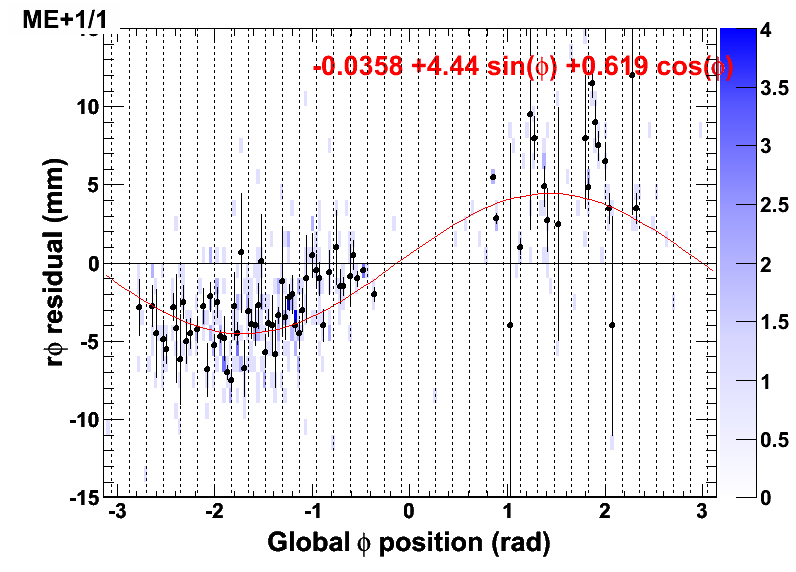
\includegraphics[width=\linewidth]{endcap_highmomentum.png}

\column{0.5\linewidth}
\begin{center}
with $p_T > 10$~GeV/$c$
\end{center}

\vspace{-0.25 cm}
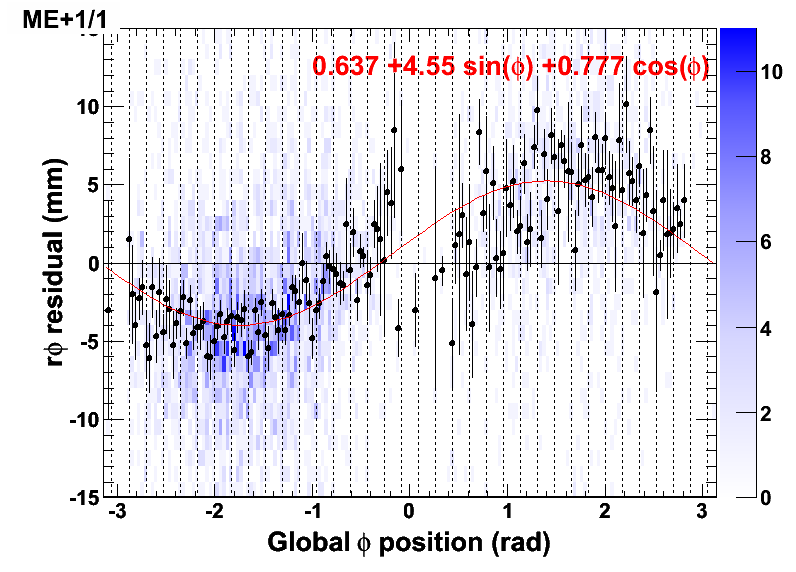
\includegraphics[width=\linewidth]{endcap_allmomenta.png}
\end{columns}

\hfill \textcolor{darkblue}{Vadim Khotilovich}
\end{frame}

\begin{frame}
\frametitle{Today's schedule}

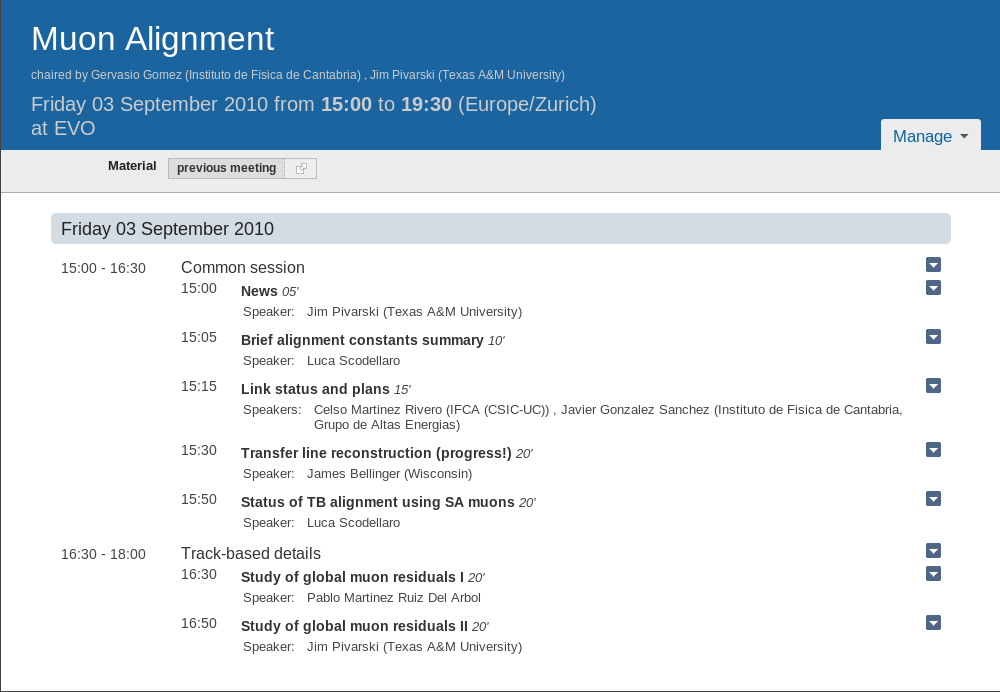
\includegraphics[width=\linewidth]{schedule.png}
\label{numpages}
\end{frame}

\end{document}
